\documentclass[tikz,border=8pt]{standalone}
% Shared look for every TikZ diagram. Load with \input{../../tools/tikz-style.tex}
\usepackage[T1]{fontenc}
\usepackage{lmodern}
\renewcommand{\sfdefault}{lmr}  % diagrams use the same serif as the text
\usetikzlibrary{arrows.meta, positioning, shapes.geometric, calc, fit, backgrounds}
\definecolor{cblue}{HTML}{4C78A8}
\definecolor{corange}{HTML}{F58518}
\definecolor{cgreen}{HTML}{54A24B}
\definecolor{cred}{HTML}{E45756}
\definecolor{cpurple}{HTML}{B279A2}
\definecolor{cgrey}{HTML}{6B6B6B}
\tikzset{
  every picture/.style={font=\sffamily, line width=1.2pt},
  box/.style={draw=#1, fill=#1!12, rounded corners=4pt, align=center, inner sep=7pt, minimum height=1.1cm},
  box/.default=cgrey,
  arrow/.style={-{Stealth[length=3mm]}, draw=cgrey, line width=1.4pt},
  title/.style={font=\sffamily\bfseries\Large},
  note/.style={font=\sffamily\small, text=cgrey, align=center},
}
\AtBeginDocument{\hyphenpenalty=10000 \exhyphenpenalty=10000}

\begin{document}
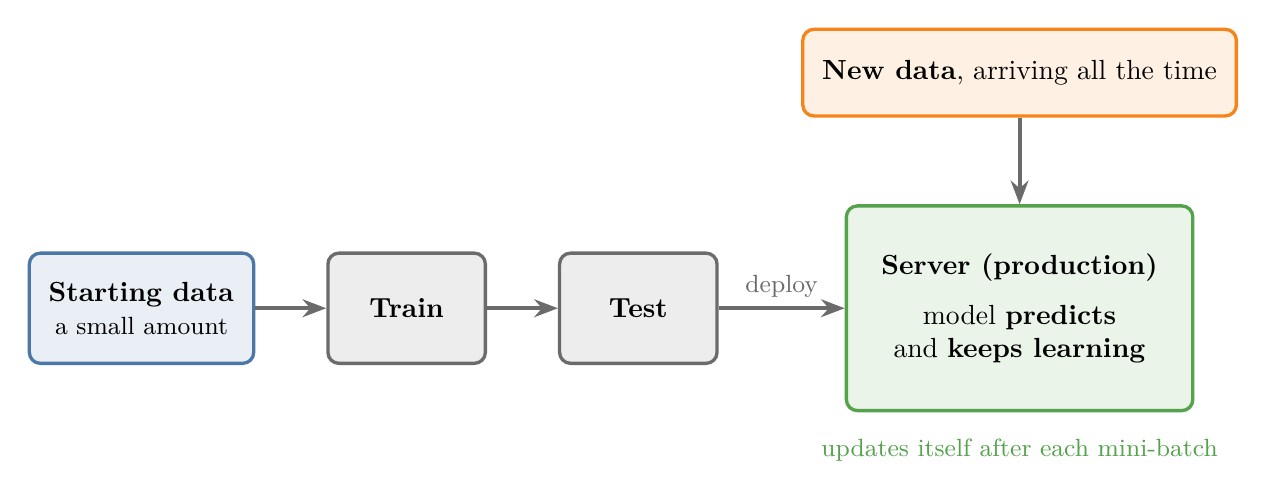
\begin{tikzpicture}[node distance=0.9cm]
  \node[box=cblue, minimum width=2.4cm, minimum height=1.4cm] (data) {\textbf{Starting data}\\{\small a small amount}};
  \node[box=cgrey, right=of data, minimum width=2.0cm, minimum height=1.4cm] (train) {\textbf{Train}};
  \node[box=cgrey, right=of train, minimum width=2.0cm, minimum height=1.4cm] (test) {\textbf{Test}};
  \node[box=cgreen, right=1.6cm of test, minimum width=4.4cm, minimum height=2.6cm, align=center] (server)
    {\textbf{Server (production)}\\[6pt]model \textbf{predicts}\\and \textbf{keeps learning}};
  \draw[arrow] (data) -- (train); \draw[arrow] (train) -- (test); \draw[arrow] (test) -- node[note, above] {deploy} (server);
  \node[box=corange, above=1.1cm of server, minimum width=4.4cm] (new) {\textbf{New data}, arriving all the time};
  \draw[arrow] (new) -- (server);
  \node[note, text=cgreen, below=0.2cm of server] {updates itself after each mini-batch};
\end{tikzpicture}
\end{document}
